\documentclass[12pt, a4paper]{article}
\edef\restoreparindent{\parindent=\the\parindent\relax}
\usepackage{fontspec}
\usepackage{amsmath}
\usepackage[UKenglish]{babel}
\usepackage[bibstyle=ieee, dashed=false, sorting=nty]{biblatex}
\usepackage[labelfont=bf]{caption}
\usepackage{csquotes}
\usepackage{fancyhdr}
\usepackage{float}
\usepackage[top=30mm, right=25mm, bottom=30mm, left=25mm]{geometry}
\usepackage[hidelinks]{hyperref}
\usepackage{listings}
\usepackage{mhchem}
\usepackage{microtype}
\usepackage{parskip}
\usepackage[dvipsnames]{xcolor}
\usepackage{tikz}

\restoreparindent

\lstset{captionpos=b, columns=flexible}
\usetikzlibrary{fpu, positioning, shapes}

\pagestyle{fancy}
\fancyhf{}
\fancyhead[L]{COM3190}
\fancyhead[C]{Assignment: Simulating Chemistry}
\fancyhead[R]{160203853}
\fancyfoot[C]{\thepage}

\addbibresource{references.bib}

\begin{document}

\section{CCS Model}
\subsection{Problems of Default CCS Model Definiton} \label{subsec:default_problems}
\begin{enumerate}
  \item \textbf{Livelock scenario:} The would happen when the system has at least one $O$
  and $OH$ spawned. $O$ can evolve into $OH$, and $OH$ can evolve into $O$, this would cause the
  system to synchronise $O$ and $OH$ continuously.
  \item \textbf{Deadlock scenario:} By working through the CCS processes manually, the system will
  reach a state where it would require to synchronise on either an $o$ or $h$ in order to evolve two
  of the processes. However, in order for two processes to synchronise on $o$, the system must at
  least synchronise on $h$ before. This introduces a deadlock because $o$ and $h$ have mutual
  dependency.
\end{enumerate}

\subsection{Improved CCS Model}
The objective is to eliminate the problems stated in
\hyperref[subsec:default_problems]{\textbf{Section \ref*{subsec:default_problems}}}. The accepted
intermediate states are: $CH_3, CH_4, HCO, CH_3O, CH_2OH$. The rule highlighted in bold is added to
ensure that the system can simulate the equation \hyperref[equation:one]{(\ref*{equation:one})}.

\begin{align*}
  CH_3OH \; &= \; \overline{c}.(H_2 \mid H \mid OH) + \overline{h}.CH_2OH + \overline{oh}.CH_3 \\
  CH_2OH \; &= \; \overline{c}.(H \mid H \mid OH) + \overline{h}.(COH \mid H) + \overline{oh}.(C \mid H_2) \\
  COH \; &= \; \overline{c}.OH + \overline{oh}.C \\
  \\
  CH_3 \; &= \; \overline{c}.(H_2 \mid H) + \overline{h}.(C \mid H_2) \\
  \\
  H_2 \; &= \; \boldsymbol{o.H_2O} + \overline{h}.H \\
  H \; &= \; oh.H_2O + \overline{h}.0 \\
  \\
  O_2 \medspace \; &= \; c.CO_2 + \overline{o}.O \\
  O \; &= \; h.OH + \overline{o}.0 \\
  OH \; &= \; h.H_2O + \overline{o}.H \\
  C \; &= \; o.CO \\
  CO \; &= \; o.CO_2
\end{align*}

\section{Erlang Implementation}
\subsection{Design} \label{sec:design}
It is known that a complete combustion of methanol in oxygen will form carbon dioxide and water,
which is described as the balanced equation below:
\begin{equation}
  \ce{2CH3OH + 3O2 -> 2CO_2 + 4H_2O} \label{equation:one}
\end{equation}

The primary objective of the Erlang implementation is to simulate the equation
\hyperref[equation:one]{(\ref*{equation:one})}. The system needs to satisfy the requirements below:
\begin{enumerate}
  \item When the ratio of \ce{CH3OH} to \ce{O2} is 2 to 3, the system must undergo complete
  combustion and produce \ce{CO2} and \ce{H2O} of ratio 2 to 4.
  \item When the ratio of \ce{CH3OH} to \ce{O2} is \textbf{not} 2 to 3, the system will undergo
  incomplete combustion and produce incomplete amount of \ce{CO2} and \ce{H2O}, along with some
  intermediate products.
  \item At the end of the reaction, the system must be able to detect whether it is a complete or
  incomplete combustion.
\end{enumerate}

\subsection{Program Flow Diagram}
\begin{figure}[H]
  \centering
  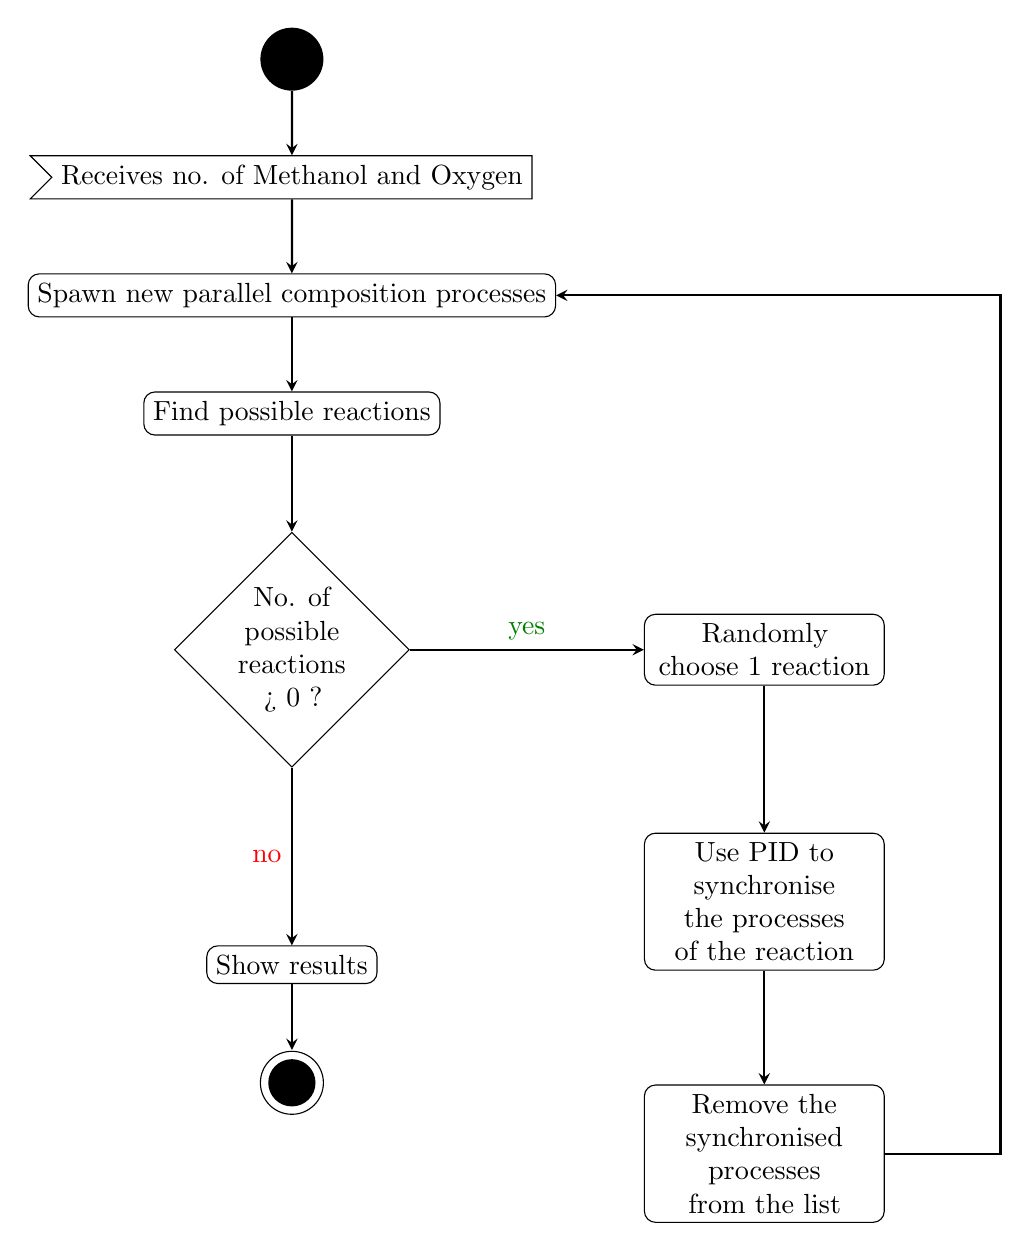
\begin{tikzpicture}
    [node distance=1.5cm,
    start/.style={circle, fill=black, minimum size=8mm},
    end/.style={path picture={\draw circle [radius=4mm]; \fill circle [radius=3mm];},minimum
    size=8.2mm},
    activity/.style={rectangle, draw, text centered, rounded corners},
    decision/.style={diamond, draw, text width=4em, text badly centered, inner sep=0pt,
    node distance=2.5cm},
    input/.style={signal, draw, signal from=west, signal to=nowhere},
    output/.style={signal, draw, signal to=east},
    arrow/.style={thick, ->, >=stealth}]
    \node [start] (start) {};
    \node [input, below of=start] (react) {Receives no. of Methanol and Oxygen};
    \node [activity, below of=react] (spawn) {Spawn new parallel composition processes};
    \node [activity, below of=spawn] (find_reaction) {Find possible reactions};
    \node [decision, below of=find_reaction, node distance=3cm] (has_reactions) {No. of possible
    reactions > 0 ?};
    \node [activity, right of=has_reactions, text width=8em, node distance=6cm] (random)
    {Randomly choose 1 reaction};
    \node [activity, below of=random, text width=8em, node distance=3.2cm] (perform) {Use PID to
    synchronise the processes of the reaction};
    \node [activity, below of=perform, text width=8em, node distance=3.2cm] (remove) {Remove the
    synchronised processes from the list};
    \node [activity, below of=has_reactions, node distance=4cm] (show_results) {Show results};
    \node [end, below of=show_results] (end) {};

    \draw [arrow] (start) -- (react);
    \draw [arrow] (react) -- (spawn);
    \draw [arrow] (spawn) -- (find_reaction);
    \draw [arrow] (find_reaction) -- (has_reactions);
    \draw [arrow] (has_reactions.east) -- node [anchor=south] {\textcolor{Green}{yes}} (random.west)
    ;
    \draw [arrow] (random) -- (perform);
    \draw [arrow] (perform) -- (remove);
    \draw [arrow] (remove) -- ++ (3,0) |- (spawn);
    \draw [arrow] (has_reactions) -- node [anchor=east] {\textcolor{Red}{no}} (show_results);
    \draw [arrow] (show_results) -- (end);
  \end{tikzpicture}
  \caption{Flow diagram of the Erlang implementation}
  \label{figure:program_flow}
\end{figure}

\subsection{Implementation Details}
This section will discuss design concepts and implementation details of the system to provide
explanation for the program flow in \hyperref[figure:program_flow]{\textbf{Figure
\ref*{figure:program_flow}}}.

\subsubsection{Rule set}
In the Erlang implementation, process synchronisation is done by sending and receiving messages
through process identifier (PID). The system itself does not know which processes could synchronise
with each other. Therefore, a rule set must be integrated to allow the system to check for possible
reactions.

\begin{lstlisting}[language=erlang, label=code:rule_set,xleftmargin=.2\textwidth,
  xrightmargin=.2\textwidth, caption=A rule set definition in Erlang maps \cite{erlang_maps}]
  Rules = #{
    ch3oh => [{snd, c}, {snd, h}, {snd, oh}],
    ch2oh => [{snd, c}, {snd, h}, {snd, oh}],
    coh => [{snd, c}, {snd, oh}],
    ...
    o2 => [{rcv, c}, {snd, o}],
    ...
  },
\end{lstlisting}

A partial rule set is shown in \hyperref[code:rule_set]{\textbf{Listing \ref*{code:rule_set}}}. The
atom \texttt{snd} and \texttt{rcv} represent `send' and `receive' respectively. For two processes to
synchronise, one must be able to `\texttt{snd}', and the other must be able to `\texttt{rcv}' the
same atom. The system will use this mechanism to find possible reactions. For instance,
\texttt{ch3oh}, \texttt{ch2oh}, \texttt{coh} can `\texttt{snd}' a \texttt{c}, and \texttt{o2} can
`\texttt{rcv}' a \texttt{c}. Hence, the system will know that \texttt{ch3oh}, \texttt{ch2oh}, and
\texttt{coh} can all synchronise with \texttt{o2}.

\subsubsection{Reactants List}
Moreover, the system also needs to have a variable to store the reactants (processes spawned) left.
The reactants list is used by the system to find possible reactions, and to determine whether the
reaction has ended. The reactants list store a list of reactants in the form \texttt{\{atom, PID\}},
where \texttt{atom} represents the name of the reactant, and \texttt{PID} represents the process
identifier of the reactant.

\begin{lstlisting}[basicstyle=\ttfamily, label=code:reactants_list,
  caption=An example of reactants list.]
  [{ch3oh,<0.98.0>},{h,<0.106.0>},{o2,<0.99.0>},{oh,<0.107.0>},...]
\end{lstlisting}

\subsubsection{Initialising the Start Process} \label{subsubsec:start}
Since the system should only terminate when there are no possible reactions left, and synchronising
two processes would generally involve spawning processes as well, a start process is implemented to
handle the main logic of the system based on \hyperref[figure:program_flow]{\textbf{Figure
\ref*{figure:program_flow}}}. The start process is initially registered when the user has provide
the number of Methanol and Oxygen molecules, and it is kept alive until the end of the reaction. It
is a recursive function, the new processes spawned after a synchronisation are sent back, and then
it will start to find possible reactions again.

\begin{lstlisting}[language=erlang, basicstyle=\small, label=code:start_reaction,
  caption=A function that handles the main logic of the system]
-spec start_reaction([{atom(), pid()}]) -> none().
% @doc Main logic, start the combustion of methanol
% @param Reactants The list of reactants

start_reaction(Reactants) ->
  Reaction = find_reaction(Reactants),
  case Reaction of
    % No possible reactions left, end and show results
    [] -> result ! {finished, Reactants};

    % Randomly chosen reaction returned
    {{R1, _}, {R2, _}, _} ->
      perform_reaction(Reaction),

      % Remove the two reactants reacted after the reaction
      NewReactants = remove_reactants(R1, R2, Reactants),

      % Wait until the reaction has finished, then repeat again
      receive
        NewProcesses ->
          start_reaction(lists:merge(NewProcesses, NewReactants))
      end
  end.
\end{lstlisting}

\subsubsection{Finding Possible Reactions}
With the rule set and reactants list defined, the system can now find possible reactions in the
reactants list. Given a reactants list, the system will process the list recursively, searching for
reactants that can synchronise with each other. All possible reactions will be stored in a list in
the format shown in \hyperref[code:reaction_type]{\textbf{Listing \ref*{code:reaction_type}}}. In
order to simulate the `randomness' behaviour of chemistry and the `choice' behaviour of CCS, the
reaction to perform will be randomly selected from the list of possible reactions. If no possible
reactions are found, then this indicates that the reaction has ended, and the system will show the
results.

\begin{lstlisting}[basicstyle=\ttfamily, label=code:reaction_type,
  caption=An example of a possible reaction,xleftmargin=.13\textwidth]
  {{{ch3oh, <0.98.0>}, snd}, {{o2, <0.99.0>}, rcv}, c}
\end{lstlisting}

\subsubsection{Synchronising Processes} \label{subsubsec:sync}
After finding a reaction to perform, the system will then simulate the `synchronisation' behaviour.
According to \hyperref[code:reaction_type]{\textbf{Listing \ref*{code:reaction_type}}}, all the
required information to perform the synchronisation has been recorded. Using
\hyperref[code:reaction_type]{\textbf{Listing \ref*{code:reaction_type}}} as an example, the system
can extract the following information:
\begin{enumerate}
  \item \texttt{ch3oh} can synchronise with \texttt{o2} on \texttt{c}
  \item The PID of \texttt{ch3oh}
  \item The PID of \text{o2}
  \item \texttt{ch3oh} is the sender
  \item \texttt{o2} is the receiver
\end{enumerate}

Since \texttt{ch3oh} is the sender, it should send \texttt{c} to \texttt{o2} and
evolve. However, in Erlang implementation, the \texttt{ch3oh} process itself does not know its
identity. Therefore, the system must first send a message to \texttt{ch3oh}, telling it to send
\texttt{c} to the PID of \texttt{o2} in order to synchronise the processes. The function to initiate
the synchronisation process is shown in \hyperref[code:perform_reaction]{\textbf{Listing
\ref*{code:perform_reaction}}}.

\begin{lstlisting}[language=erlang, basicstyle=\footnotesize, label=code:perform_reaction,
  caption=A function to perform the reaction]
-spec perform_reaction(reaction()) -> none().
% @doc Perform a reaction
% @param A reaction

perform_reaction({{{R1, R1_Pid}, R1_Comm}, {{R2, R2_Pid}, R2_Comm}, Action}) ->
  case {R1_Comm, R2_Comm} of
    {snd, rcv} ->
      % Reactant 1 sends Action to Reactant 2
      R1_Pid ! {snd, Action, R2_Pid},
    {rcv, snd} ->
      % Reactant 2 sends Action to Reactant 1
      R2_Pid ! {snd, Action, R1_Pid},
  end.
\end{lstlisting}

\subsubsection{Evolving and Spawning New Processes}
\begin{lstlisting}[language=erlang, basicstyle=\small,numbers=left,label=code:reactants,
  caption=Partial code listing of \texttt{ch3oh} and \texttt{o2}]
ch3oh() ->
  receive
    {snd, c, To} ->
      To ! {rcv, c, ch3oh, self()},
      receive
        {ok, R} -> start ! spawn_reactants([h2, h, oh] ++ R)
      end;
    ...
  end.

o2() ->
  receive
    {rcv, c, From, Pid} ->
      co2(),
      Pid ! {ok, []};
    ...
  end.
\end{lstlisting}

In Erlang, message sending is asynchronous \cite{message_sending}. For example, in
\hyperref[code:reactants]{\textbf{Listing \ref*{code:reactants}}}, after \texttt{ch3oh} has sent a
\texttt{c} to \texttt{o2}, it will then wait for a response from \texttt{o2} (line 6). The response
message will contain \texttt{ok}, along with a list of new processes to spawn (line 15, in this case
the list is empty because \ce{O2} has become \ce{CO2}). As mentioned in
\hyperref[subsubsec:start]{\textbf{Section \ref*{subsubsec:start}}}, new processes spawned after the
synchronisation will be sent back to the start process (line 6). After that, the synchronisation is
considered complete and the system can proceed to find new possible reaction.

\subsubsection{Traces}
In order to prove that the system implemented matches the CCS model, one possible trace of the
system is shown in \hyperref[traces]{\textbf{Listing \ref*{traces}}}. It has been shown that the
processes synchronised are removed from the reactants list, and new processes spawned are added into
the reactants list. Moreover, \hyperref[traces]{\textbf{Listing \ref*{traces}}} has also shown that
the system has fulfilled the requirements set in \hyperref[sec:design]{\textbf{Section
\ref*{sec:design}}}.

\begin{lstlisting}[basicstyle=\ttfamily\small, label=traces,caption=Traces of the system]
> chemistry:react(4,2).

Reactants left: [ch3oh,ch3oh,ch3oh,ch3oh,o2,o2]
ch3oh --c--> o2
o2 <--c-- ch3oh

Reactants left: [ch3oh,ch3oh,ch3oh,h2,h,o2,oh]
ch3oh --h--> oh
oh <--h-- ch3oh

Reactants left: [ch2oh,ch3oh,ch3oh,h2,h,o2]
ch2oh --c--> o2
o2 <--c-- ch2oh

Reactants left: [ch3oh,ch3oh,h,h,h2,h,oh]
ch3oh --h--> oh
oh <--h-- ch3oh

Reactants left: [ch2oh,ch3oh,h,h,h2,h]
ch2oh --oh--> h
h <--oh-- ch2oh

Reactants left: [c,ch3oh,h,h,h2,h2]
ch3oh --oh--> h
h <--oh-- ch3oh

Reactants left: [c,ch3,h,h2,h2]
Final products: 2CO2 + 4H2O + 2H2 + 1C + 1CH3 + 1H
Status        : Run out of O2
-------------------------------------------------------------------
> chemistry:react(2,3).

Reactants left: [ch3oh,ch3oh,o2,o2,o2]
ch3oh --c--> o2
o2 <--c-- ch3oh

Reactants left: [ch3oh,h2,h,o2,o2,oh]
ch3oh --h--> oh
oh <--h-- ch3oh

Reactants left: [ch2oh,h2,h,o2,o2]
ch2oh --oh--> h
h <--oh-- ch2oh

Reactants left: [c,h2,h2,o2,o2]
o2 --o--> c
c <--o-- o2

Reactants left: [h2,h2,o,co,o2]
o --o--> h2
h2 <--o-- o

Reactants left: [h2,co,o2]
o2 --o--> h2
h2 <--o-- o2

Reactants left: [co,o]
o --o--> co
co <--o-- o

Reactants left: []
Final products: 2CO2 + 4H2O
Status        : Complete combustion
\end{lstlisting}

\subsection{Testing}
EUnit testing has been done to cover the functionalities of some helper functions.

\begin{lstlisting}[basicstyle=\ttfamily\small,caption=EUnit testing]
> chemistry_test:test().
  All 42 tests passed.
ok
\end{lstlisting}

\subsection{Conclusion}
\begin{enumerate}
  \item The system implemented is functional, and is able to meet the requirements set.
  \item The system is able to simulate the `randomness' behaviour of chemistry reaction, as well as
  the CCS choices behaviour by randomly selecting one reaction from a list of possible reactions.
  \item Erlang is able to simulate the CCS synchronisation by message sending and receiving between
  processes.
  \item Different definitions of CCS model may produce different results on the same input.
\end{enumerate}

\printbibliography

\appendix
\section*{Appendix}
\subsection*{Default CCS Definition}
\begin{align*}
  CH_3OH \; &= \; \overline{c}.H_3OH + \overline{h}.CH_2OH + \overline{oh}.CH_3 \\
  CH_2OH \; &= \; \overline{c}.H_2OH + \overline{h}.CHOH + \overline{oh}.CH_2 \\
  CHOH \; &= \; \overline{c}.HOH + \overline{h}.COH + \overline{oh}.CH \\
  COH \; &= \; \overline{c}.OH + \overline{oh}.C \\
  \\
  CH_3 \; &= \; \overline{c}.H_3 + \overline{h}.CH_2 \\
  CH_2 \; &= \; \overline{c}.H_2 + \overline{h}.CH \\
  CH \; &= \; \overline{c}.H + \overline{h}.C \\
  \\
  H_3OH \; &= \; \overline{h}.H_2OH + \overline{oh}.H_3 \\
  H_2OH \; &= \; \overline{h}.HOH + \overline{oh}.H_2 \\
  HOH \; &= \; \overline{h}.OH + \overline{oh}.H \\
  \\
  H_3 \; &= \; \overline{h}.H_2 \\
  H_2 \; &= \; \overline{h}.H \\
  H \; &= \; oh.H_2O + \overline{h}.0\\
  \\
  O_2 \; &= \; c.CO_2 + \overline{o}.O \\
  O \; &= \; h.OH + \overline{o}.0 \\
  OH \; &= \; h.H_2O + \overline{o}.H + \overline{h}.O \\
  C \; &= \; o.CO \\
  CO \; &= \; o.CO_2
\end{align*}

\end{document}
